\documentclass[a4paper,10pt]{article}
\usepackage[utf8]{inputenc}
\usepackage{rotating}
\usepackage{comment}
\usepackage{acronym}
\usepackage{tikz}
\usepackage{multirow}


\usetikzlibrary{fit,arrows}


\acrodef{nfs}[NFS]{Network File-System}
\acrodef{bot}[BoT]{Bag of Tasks}
\acrodef{omssa}[OMSSA]{Open Mass-Spectrometry Search Algorithm}
\acrodef{vm}[VM]{virtual machine}
\acrodef{btu}[BTU]{\emph{billing time unit}}
\acrodef{asap}[ASAP]{\emph{as soon as possible}}
\acrodef{afap}[AFAP]{\emph{as full as possible}}

%opening
\title{Cloud simulation}
\author{}

\usepackage{graphicx}

\newcommand\vrpath{../../lab/setup/simschlouder/validation-results/}
\graphicspath{{\vrpath}}

\begin{document}

\maketitle

\begin{abstract}

Simulating the cloud from the client point of view.

Assessment of the impact of different metrics.

Recommendations for using cloud simulators.

WARNING: figures in text might not be up to date.

\end{abstract}

\section{Introduction}





The  problem   of  allocating   cloud  resources   in  performant,   robust  and
energy-efficient ways is  of paramount importance in today's  usage of computing
infrastructures, and a number of research papers have contributed new allocation
techniques to  address this issue.   A pitfall of research  on IaaS lies  in the
validation of the models and algorithms proposed, which requires infrastructures
that are difficult to set up for individual researchers.  As a consequence, many
researchers evaluate their work through  simulation. A number of simulators have
been  developed for  that purpose  (\cite{9-14}).  They  are typically  based on
discrete-event simulation,  using models  for each  elementary component  of the
infrastructure,  which  are then  composed  to  simulate  the whole  system  and
applications running on it.  This approach is attractive from the infrastructure
provider  perspective  since the  simulated  system  can be  finely  customized.
However, such  an \textit{ab  initio} construction  poses a  significant problem
regarding  the  calibration  and  validation   of  the  composed  model  against
real-world  measurements.    Another  approach   is  the  simulation   from  the
client-side (from the application perspective),  which can specifically focus on
the prediction of a couple of metrics, such  as the makespan and the cost of the
application.  It  is noticeable  that the research  adopting a  client-side view
generally evaluate the  accuracy of their simulation  model through experimental
studies, while such  an evaluation is generally  missing for infrastructure-wide
simulators.

Altough much  fewer works  address the simulation  from the  client perspective,
several very  different methods have  been proposed  to reach this  goal.  Among
these    works,     detailed    in    the    related     work    section,    are
EMUSIM~\cite{CalheirosNRB13}  that  use   emulation,  PICS~\cite{KimWH15}  which
implemens  a simplified  discrete  event  simulator, and~\cite{PucherGWK15}  who
build a statistical model from observations.

...


We advocate  that a precise assessment  of simulation
should be  carried out against real  execution figures to better  understand the
limits  of simulation  applicability. In  this  paper, we  study the  simulation
accuracy on several use cases ran on  an IaaS clouds. The use cases comprise two
different type  of applications (workflow  and bag-of-tasks), with  several size
instances for  each of them, and  each application is operated  on two different
type of infrastructure (private and public).


We assume an automated process  making the provisioning and scheduling decisions
on  behalf  the user  on  the  real infrastructure.   To  that  purpose, we  use
\emph{Schlouder} \cite{}, a client-side cloud resource broker.  These scheduling
algorithms of Schlouder have been reimplemented in a simulation system, based on
the simulation toolkit SimGrid~\cite{simgrid08}.   Our study aims to isolate the
different parameters that  influence the simulation accuracy and  what degree of
divergence between real execution and simulation might be expected in each case.






\begin{comment}
[9] R. N. Calheiros, R. Ranjan, A. Beloglazov, C. A. D. Rose, and R. Buyya, “CloudSim: a toolkit for modeling and simulation of cloud computing environments and evaluation of resource provisioning algo- rithms,” Software: Practice and Experience, vol. 41, no. 1, pp. 23–50,
2011.
[10] D. Kliazovich, P. Bouvry, and S. U. Khan, “GreenCloud: a packet-level simulator of energy-aware cloud computing data centers,” The Journal of Supercomputing, vol. 62, no. 3, pp. 1263–1283, 2012.

[11] B. Wickremasinghe, R. N. Calheiros, and R. Buyya, “Cloudanalyst: A CloudSim-based visual modeller for analysing cloud computing environments and applications,” in Advanced Information Networking
and Applications (AINA), 2010 24th IEEE International Conference on.
IEEE, 2010, pp. 446–452.

[12] S. K. Garg and R. Buyya, “Networkcloudsim: Modelling parallel applications in cloud simulations,” in Utility and Cloud Computing
(UCC), 2011 Fourth IEEE International Conference on. IEEE, 2011,
pp. 105–113.

[13] M. Tighe, G. Keller, M. Bauer, and H. Lutfiyya, “DCSim: A data centre simulation tool for evaluating dynamic virtualized resource management,” in Network and service management (cnsm), 2012 8th
international conference and 2012 workshop on systems virtualiztion
management (svm), Oct 2012, pp. 385–392.

[14] S. K. S. Gupta, R. Gilbert, A. Banerjee, Z. Abbasi, T. Mukherjee, and G. Varsamopoulos, “GDCSim: A tool for analyzing Green Data Center design and resource management techniques,” in Green Computing
Conference and Workshops (IGCC), 2011 International, July 2011, pp.
1–8.
\end{comment}

 
  



\section{Setup / Context}


\subsection{Real Environment}

Evaluation of simulation is done by comparing simulation logs, against logs
generated by running actual scientific workflows on multiple platforms. Though
our work on cloud scheduling and cloud simulation we acquired archive of 274
experimental executions on two wildly differing environment.

\subsubsection{Schlouder}

Every experiment log in the archive was generated by running a scientific
workflow through a client-side cloud resource broker named\emph{Schlouder}
\cite{Michon17}. \emph{Schlouder} automates the provisioning of resources needed
to execute a workflow, the scheduling of tasks to the provisioned resources and,
monitors the proper execution of tasks. 

\begin{figure}
	\centering
	\usetikzlibrary{fit,arrows}
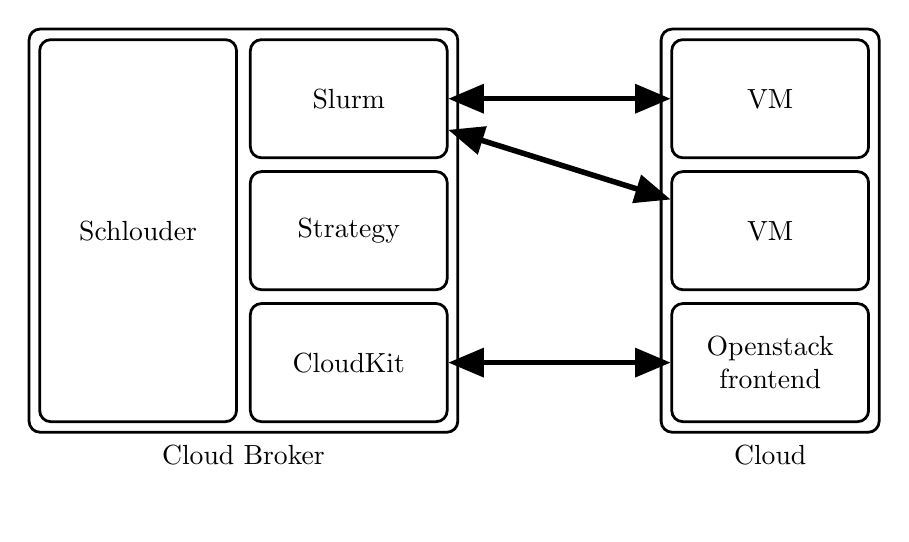
\begin{tikzpicture}[node distance=5pt,x=25mm+5pt,y=15mm+5pt,
every node/.style={anchor=center,
line width=1pt,
minimum width = 25mm,
minimum height =15mm,
rounded corners,
label distance=-5mm,
draw 
},
high/.style={%
minimum height =45mm+10pt,
},
large/.style={%
minimum width=50mm+5pt
}]
\node[high]at(0,0)(app){Schlouder};
\node[]at(1,-1)(ck){CloudKit};
\node[]at(1,0)(strat){Strategy};
\node[]at(1,1)(slm){Slurm};
\node[align=center]at(3,-1)(cc){Openstack\\frontend};
\node[]at(3,0)(vm1){VM};
\node[]at(3,1)(vm2){VM};
\node[draw,fit=(app)(ck)(slm),label={below:Cloud Broker}]{};
\node[draw,fit=(vm2)(cc)(vm1),label={below:Cloud}]{};
\draw [{triangle 45}-{triangle 45},line width=2pt] (ck)--(cc);
\draw [{triangle 45}-{triangle 45},line width=2pt] (vm2)--(slm);
\draw [{triangle 45}-{triangle 45},line width=2pt] (vm1)--(slm);
%\draw [{triangle 45}-{triangle 45},shorten <=10pt,shorten >=10pt] (1,0)--(1,1);
%\draw [{triangle 45}-{triangle 45},shorten <=10pt,shorten >=10pt] (1,0)--(1,-1);
\end{tikzpicture}

	\caption{The Schlouder cloud broker and its components relating to an
	Openstack cloud.}
\end{figure}


Provisioning is done thought a cloud kit interface that allows for Schlouder to
communicate with different clouds in order to start and stops the necessary
\acp{vm} to execute the workload.  To match account for the pricing of
commercial IaaS, Schlouder views provisioning in fixed increments of time,
referred to as \ac{btu}, machines idle when arriving at the end of their time
will be automatically shut off. 

Tasks execution is monitored using SLURM\cite{YooJG03} which connects to the
available \acp{vm}, send the jobs, and monitors their executions. 

A strategy controls provisioning and scheduling decisions, it determines when
\ac{vm} provisioned and to which \ac{vm} each task is assigned. Schlouder
provides a few basic strategies and new ones can be added trivially. Strategies
can affect the workload's \emph{makespan}, the \acp{vm} usage rate, and the
number of opened \acp{btu}(i.e.\ the price of the experiment on a commercial
cloud). The experiments in our archive mainly use two strategies, \ac{asap} and
\ac{afap}

\begin{description}
	\item[\ac{asap}] will attempt to execute tasks as early as possible by
		booting a new \ac{vm} unless a \ac{vm} is already idle or one is
		predicted to become idle faster than a \ac{vm} can boot.
	\item[\ac{afap}] will favor scheduling tasks on already opened \ac{vm}
		unless doing is predicted extend the \ac{vm} runtime by an
		additional \ac{btu}, in which case it will boot a new \ac{vm}.
\end{description}

Predicted tasks runtimes, as well as tasks dependencies, are user-provided.
Scheduling is done dynamically, as soon as tasks are submitted and all their
dependencies have been completed. Once assigned to a designated \ac{vm} jobs are
not rescheduled. However, if a \ac{vm} fails to boot Schlouder will provision a
new one to replace it.

\subsubsection{Use cases: Applications characteristics}

Two test-case applications where submitted to Schlouder in order to cover a
variety of application profiles in terms of computation intensity, data load,
and task dependency.

\subsubsection{OMSSA}

The \ac{omssa}\cite{Geer2004} comes from the field of biology, it is used in tandem mass
spectrometry analysis (also known as MS/MS analysis) to identify peptides from
the mass and fragment ions obtained by a mass spectrometer. \ac{omssa} matches
measurements from the mass spectrometer, called spectra, to a protein database.

The \ac{omssa} workload features fully independent tasks, making it \ac{bot},
since every spectra within a set can be submitted independently to \ac{omssa}.
With a \emph{communication-to-computation} ratio comprised between 20\% and \%
\ac{omssa} is considered an CPU-intensive workload.

This application was run with 4 different workload covering 2 different
mass~spectrometer resolutions of two different protein solutions, denoted
\emph{brs,hrs,brt,hrt}.

\subsubsection{Montage}

The Montage Astronomical Image Mosaic Engine\cite{montage2009} is designed to
gather astronomical images into a mosaic. This application is a workflow
designed to reproject, normalize, and collate source images into a single output
image. The montage workflow is presented figure~\ref{fig:montagewf}.

Working on images Montage is an extremely data intensive workflow with a
\emph{communication-to-computation} ratio superior to 90\%.

This application was run on images of the \emph{Pleiade} star cluster at 3
different output size, 1X1, 2X2,~and 3X3.

\begin{figure}[ht]
	\usetikzlibrary{fit,arrows}
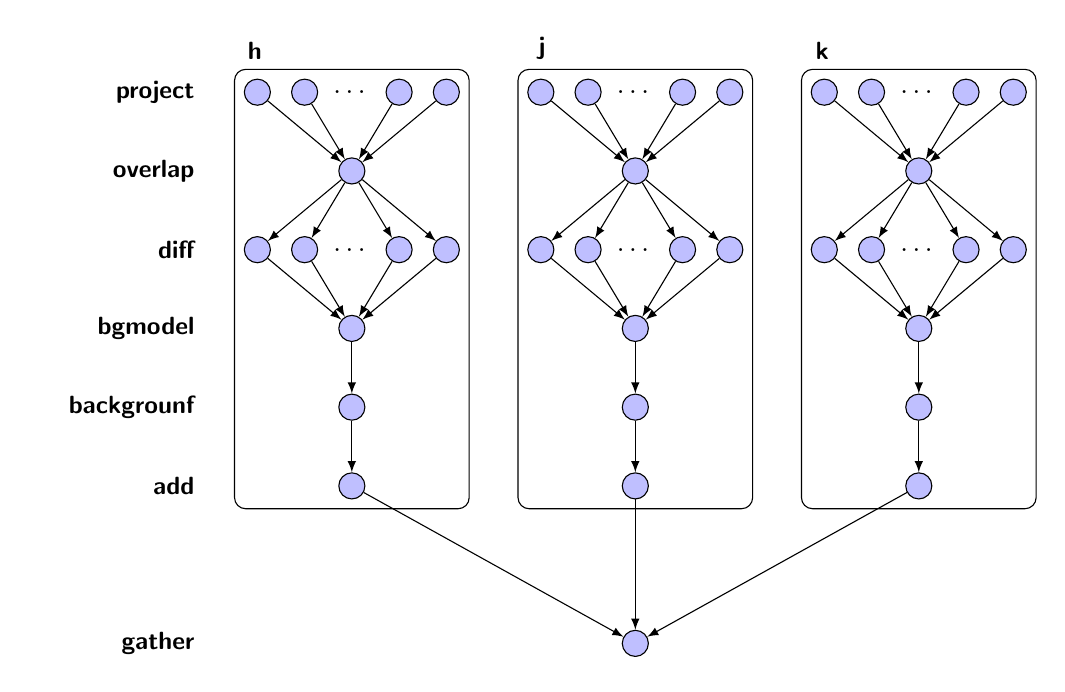
\begin{tikzpicture}[x=6mm,y=-10mm,
task/.style={%
 fill=blue!25,
draw,circle
},
level/.style={%
  font={\sffamily\bfseries\color{black} \fontsize{9pt}{12}\selectfont},
  align=right,
  text width=20mm
},
dot/.style={%
circle
}
]
%levels
\node[level] at (0,0)(Lproj){project};
\node[level] at (0,1)(Loverlap){overlap};
\node[level] at (0,2)(Ldiff){diff};
\node[level] at (0,3)(Lbgm){bgmodel};
\node[level] at (0,4)(Lbg){backgrounf};
\node[level] at (0,5)(Ladd){add};
\node[level] at(0,7)(Lgather){gather};
%%Gather node
\node[task,shift={(9,0)}]at(2,7)(gather){};
%%Loop HJK
\foreach \n [count=\i from 0] in {h,j,k}
{%
\begin{scope}[shift={(3+6*\i,0)}]
% 1 node per group
\node[task]at(2,1)(\i_overlap){};
\node[task]at(2,3)(\i_bgm){};
\node[task]at(2,4)(\i_bg){};
\node[task]at(2,5)(\i_add){};
%% 4 node per group
\foreach \y in {0,1,3,4}
{%
\node[task]at(\y,0)(\i_p_\y){};
\node[task]at(\y,2)(\i_d_\y){};
\draw[-{latex}](\i_p_\y)--(\i_overlap);
\draw[-{latex}](\i_overlap)--(\i_d_\y);
\draw[-{latex}](\i_d_\y)--(\i_bgm);
}
%%4 groups elipsis
\foreach \y in {0,2}
{%
\node[dot]at(2,\y){\ldots};
}
%%single deps
\draw[-{latex}](\i_bgm)--(\i_bg);
\draw[-{latex}](\i_bg)--(\i_add);
%%HJK boxes
\node[rounded corners,draw,fit=(\i_add)(\i_p_0)(\i_p_4),label={[font={\sffamily\bfseries\color{black}\fontsize{9pt}{12}\selectfont}]110:\n}]{};
\end{scope}
%% Gather deps
\draw[-{latex}](\i_add)--(gather);
}
\end{tikzpicture}
	\caption{Illustration of the Montage workflow. Each node represents a
	tasks and each arc represents a data dependency between two tasks. Every
	task on a specific row run the Montage command indicated on the left
	hand side of the graph.}
	\label{fig:montagewf}
\end{figure}

\subsubsection{Test beds}

The application where executed on two different clouds~: a private OpenStack
based cloud, and BonFIRE\cite{Kavoussanakis2013}, a public European cloud
testbed.

\subsubsection{Private Cloud}

Our private cloud is based on two local nodes sporting dual $2.64GHz$ Intel Xeon
processors (X5650), for a total of 96 cores. Nodes operated on Ubuntu 12.04
distributions and virtualisation is achieved using KVM. Openstack 2012.1.3 was
used as a cloud interface. This cloud was build on perfectly homogeneous nodes
and devoid of other users. For data storage these experiments rely on a
\ac{nfs}. Special attention was taken to not overbook \acp{vm} by caping the
number of single core \acp{vm} to 25. Due to the experimental nature of this
cloud configurations have change overtime. Table \ref{tab:platforms} regroups
configurations of all cloud versions. We will referrer to this cloud as
\texttt{openstack-icps.}\emph{version}.


\subsubsection{Public Cloud}

BonFire\cite{Kavoussanakis2013} is a public multi-cloud distributed all over
Europe. Our experiments were run over three sites, de-hlrs based in Stuttgart,
uk-epcc in Edinburgh, and fr-inria in Rennes. BonFIRE clouds were accessed
through an OCCI based API and the clouds were controlled throught software
derived from OpenNebula 3.6~. Each site provided different
hardware\footnote{Comprehensive information available at
\texttt{http://www.bonfire-project.eu/infrastructure/testbeds}}. Resource quotas
limited most experiment 20 \acp{vm}, not far from the limits generally
imposed on public clouds. Centralized storage was provided through a \ac{nfs}
based on the be-ibbt site in Ghent. Due to network acces restriction the
Schlouder server was brought in the BonFIRE WAN through a VPN. Due to the
experimental nature of this cloud configurations have change overtime. Table
\ref{tab:platforms} regroups configurations of all cloud versions. In this article
we refer to experiment run on the BonFire clouds by the name of the cloud site
followed by the version number.

\begin{table}
	\begin{tabular}{|l|c|c|c|c|c|c|}
		\hline
		Cloud&\#cores&Hypervisor&Network&version&\#VM&Storage\\ \hline
		\multirow{2}{*}{openstack-icps}&\multirow{2}{*}{48}&\multirow{2}{*}{KVM}&100mb&1-3&25&NFS\\\cline{4-7}
		&&&1Gb&4-5&10&NFS\\\hline
		de-hlrs&344&Xen 3.1.2&n/a&v1-3&20&NFS\\\hline
		fr-inria&96&Xen 3.2&n/a&v1-3&20&NFS\\\hline
		uk-epcc&176&Xen 3.0.3&n/a&v1-2&20&NFS\\\hline

	\end{tabular}
	\caption{Characteristics of our cloud testbeds, version numbers also
	account for changes in measured boottimes not presented in this table.}
	\label{tab:platforms}
\end{table}

\subsection{Simulations}

\subsubsection{Simulator}

SimSchlouder/SCHIaaS/Simgrid

SimSchlouder reproducing Schlouder runs. Same input/output file.

\subsubsection{Lab}

\subsubsection{Procedural Analysis}

\begin{enumerate}
 \item Real executions (xp) to test Schlouder and provisioning/scheduling 
strategies.
  Schlouder/SimSchlouder input:
  \begin{itemize}
   \item Nodes: boottime prediction, amount limit, standard power
   \item Tasks: walltime prediction
  \end{itemize}
 
 \item Normalization of xp traces (4 versions of schlouder, missing data)
 \item Extraction of information about each xp:
  \begin{itemize}
   \item Nodes: provisioning date, start date, end date, boottimes, instance 
type
   \item Tasks: submission date, scheduling date, start date, end date, 
	  walltime, input time and size, runtime, output time and size, 
management time
  \end{itemize}
 \item Simulation of each xp, injecting different information from real xps
 \item Comparison of Schlouder and SimSchlouder outputs (python)
 \item Statistical analysis of all traces (R)
 \item Close analysis of each outlier to understand the differences. 
\end{enumerate}

\subsubsection{life-cycles and observed times}

\begin{itemize}
 \item Execution: $e \in E$
 \item Node of execution $e$: $n \in N_e$
 \item Task of execution $e$: $t \in T_e$
 \item Task handled by node $n$: $t \in T_n$
 \item The node running the task $t$ is denoted $n_t \in N$
 \item $v^R$ denotes the value $v$ in the rality
 \item $v^S$ denotes the value $v$ in the simulation
 \item 
\end{itemize}

During the execution, the node are in the following states:
\begin{enumerate}
 \item Future: Once the decision to start the node is made;
 \item Pending: Once the node is requested to the cloud-kit;
 \item Booting: Once the cloud-kit aknowledge the satisfaction of the request;
 \item Idle: Once the node is ready to run tasks;
 \item Busy: Once the node is running one task;
 \item ShuttingDown: Once the termination of the node is aked to the cloud-kit;
 \item Terminated: Once the node is terminated.
\end{enumerate}

The observed times are:
\begin{itemize}
 \item $uptime(n) = terminated_n - booting_n$ 
 \item $boottime(n) = idle_n - booting_n$ 
\end{itemize}


During the execution, the task are in the following states, each corresponding to one date:
\begin{enumerate}
 \item Pending: Once they are subitted to the system;
 \item Scheduled: Once the system decided on which node the taks should be executed;
 \item Submitted: Once the task is sent to the worker node;
 \item Inputting: Once the task begin to download its data;
 \item Running: Once the task begin to computed;
 \item Outputting: Once the task begin to upload its result;
 \item Finished: Once the task is finished;
 \item Complete: Once the system aknowledge the completion of the task.;
\end{enumerate}

The observed times are:
\begin{itemize}
 \item $walltime(t) = complete_t - submitted_t$ 
 \item $inputtime(t) = running_t - inputting_t$
 \item $runtime(t) = outputting_t - running_t$
 \item $outputtime(t) = finished_t - outputting_t$
 \item $managementtime(t) = walltime_t - (inputtime_t+runtime_t+outputtime_t)$
 \item or $managementtime(t) = (inputting_t - submitted_t) + (complete_t - finished_t)$
\end{itemize}



\section{Results}

\subsection{Definitions}
4 metrics $m \in M$ for each execution $e \in E$:
\begin{itemize}
 \item uptime: amount of rented resources, cost 
  $$uptime(e) = \sum_{n \in N_e} uptime_n$$
 \item makespan: duration of the xp from the submission of the first task to 
the end of the last task, user experience 
  $$makespan(e) = max_{t \in T_e} complete_t$$
 \item usage: runtime / uptime, efficiency of the provisioning 
  $$usage(e) = \frac{\sum_{t \in T_e} walltime_t}{\sum_{n \in N_e} uptime_n}$$
 \item schederror: number of tasks that are not assigned to the same node in 
the simulation compared to the reality, accuracy of the scheduling decisions
  $$schederror(e) = |t \forall t \in T / t_n^R \neq t_n^S|$$

\end{itemize}

Absolute errors are computed for each metric $m \in M$: 
$$m.ae(e) = \frac{| m^S(e) - m^R(e) |}{m^R(e)}$$

Results are shown as frequencies and statistics (stat = min, mean, median, max) 
of absolute errors occurrences. Frequencies are weighted so that the two applications
weigth the same, and the two platforms weigth alos the same 
(i.e. each couple application $\times$ platform represents 1/4th of the frequencies).

To compare absolute errors between set of simulations $S$ and $S'$
$S$ being the reference:
\begin{itemize}
 \item $\delta stat(m.ae(E)) = stat_{e \in E} ( m.ae^{S'}(e) ) - stat_{e \in E}( m.ae^S(e) )$
 \item $\Delta stat(m.ae(E)) = stat_{e \in E} ( m.ae^{S'}(e) - m.ae^S(e) )$
\end{itemize}




\subsection{Simulator accuracy}

Best simulation we can do.

Assess the raw simulator accuracy, injecting all real-life hazards that can be 
captured :
boottimes, walltimes and scheduling dates.

Scheduling dates allow to simulate some internal threaded mechanisms of 
Schlouder.
Schlouder uses two threads: the node manager and the task manager.
At settled intervals, the node manager interrupts the task manager to start and 
stop new nodes.
This changes the state of nodes, which influence provisioning and scheduling 
decisions.
However, simulating the exact moment of this interruption is utterly difficult, 
leading to differences between simulation and reality.


\begin{figure}
  \centering

  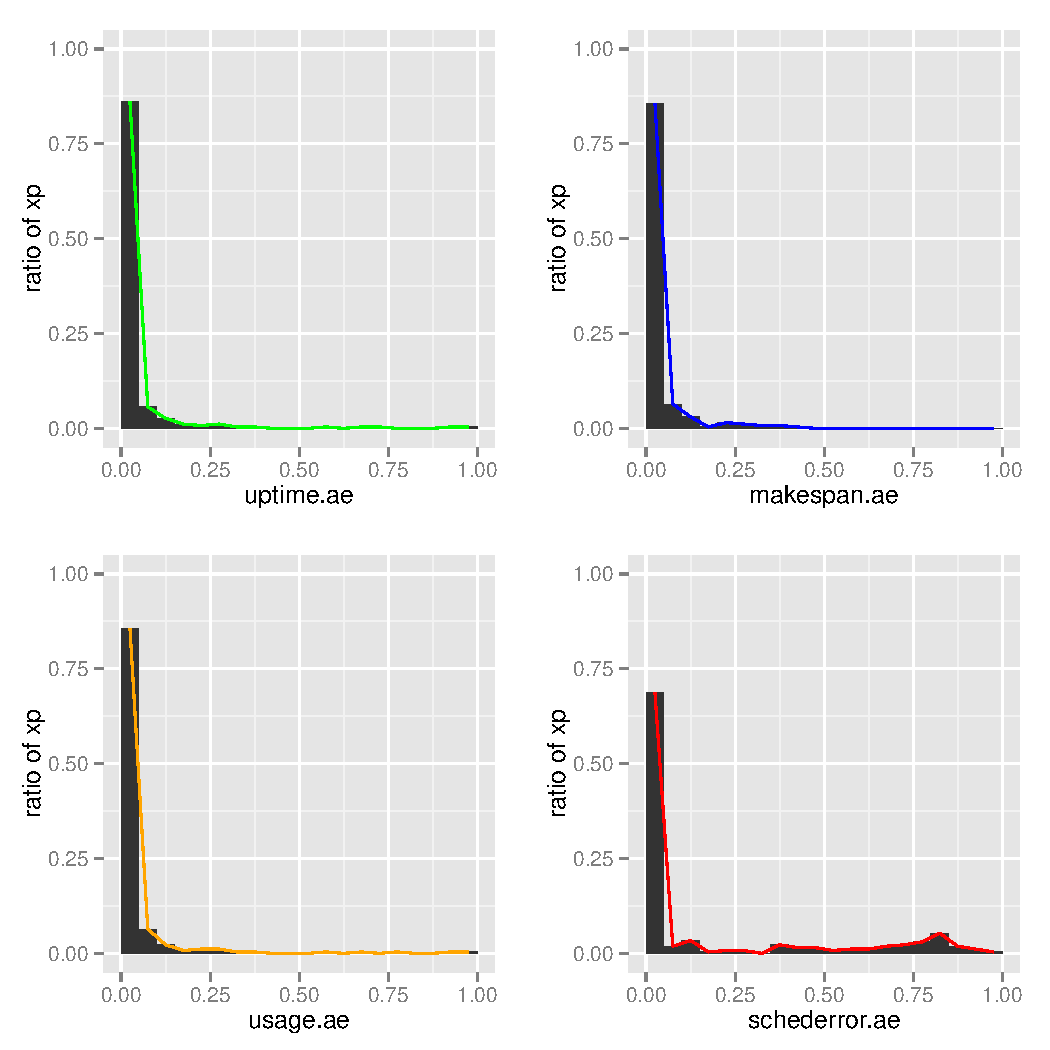
\includegraphics[width=\textwidth]{sim_best-4metrics.pdf}
  
  \input{\vrpath sim_best-4metrics-mmmm.latex}
  
\caption{Frequencies and statistics about absolute error of best simulations (274 xp)}
\end{figure} 

 


% see schiass/lab/setup/simschlouder/validation-results/best-4metrics.dat
\begin{itemize}
 \item uptime: 
      86\% show less than $0.05$ of absolute error, 
      92\% less than $0.10$, 
      2 simulations exceed $0.30$,
      ranging from $0.00$ to $0.50$, for a mean of $0.025$ and a median of $0.001$
 \item makespan: 
      76\% show less than $0.05$ of absolute error, 
      90\% less than $0.10$, 
      0 simulations exceed $0.30$,
      ranging from $0.00$ to $0.62$, for a mean of $0.042$ and a median of $0.018$
 \item usage: 
      59\% show less than $0.05$ of absolute error, 
      91\% less than $0.10$, 
      2 simulations exceed $0.30$,
      ranging from $0.00$ to $0.60$, for a mean of $0.043$ and a median of $0.002$
 \item schederror: 
      70\% show less than $0.05$ of absolute error, 
      72\% less than $0.10$, 
      59 simulations exceed $0.30$,
      ranging from $0.00$ to $0.965$, for a mean of $0.155$ and a median of $0.000$
\end{itemize}

If global metrics are quite accurately assessed by the simulator, 
the scheduling decisions can be very different between simulation and reality. 
One part of the explanation is that scheduling decisions are interdependent: 
any error leads to several others.


\subsection{Simulator accuracy according to platforms and applications}


\begin{figure}
  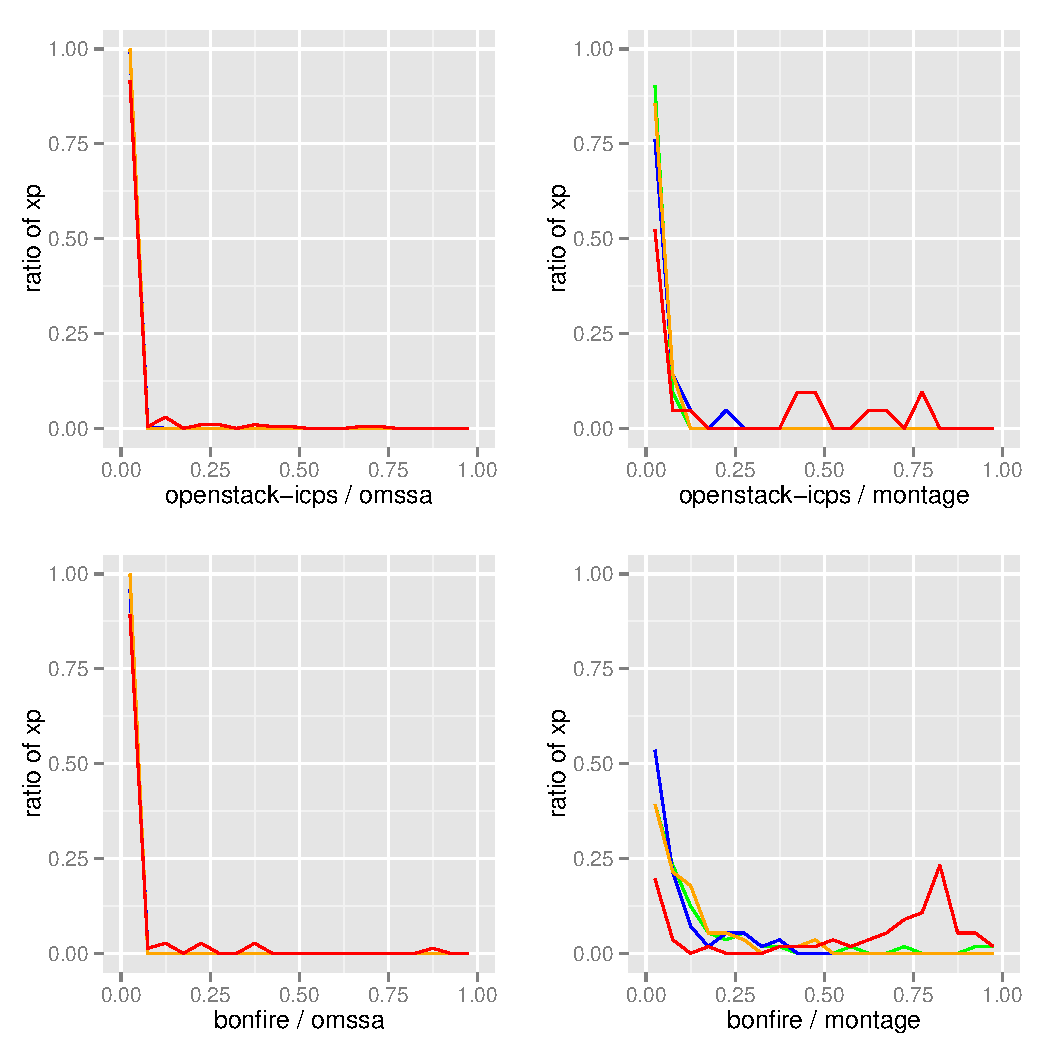
\includegraphics[width=\textwidth]{sim_best-4metrics-platform-app.pdf}
\caption{Absolute error frequencies of best simulations according to platforms 
and applications}
\end{figure} 

\begin{itemize}
 \item openstack-icps / omssa (107 xp): 
 
      \input{\vrpath sim_best-openstack-icps-omssa-4metrics-mmmm.latex}
 
      All metrics are almost perfectly assessed (mean AR from $0.001$ to $0.002$)
      except scheduling error 
      (mean $0.04$ and max $0.75$, 13\% of xp show at least one error), 
      leading to small makespan and usage errors. 
      
      We looked at each single case of scheduling error and all those errors 
      comes from ambiguities in the scheduling algorithms.
      
      This is a first limitation of simulation:
      Whenever heuristics lead to several equivalent solutions, 
      the decision is made by the implementation and relies on data structures 
      (e.g. selection of the first encountered suitable solution) or clocks 
      (e.g. the solution differs from a second to the next, which depends 
      on threads activations and timers). While we made sure to use the same 
      structures and timers, some clocks-related events can not be captured nor 
      simulated: Processing the nodes and tasks queues for scheduling and 
      provisioning decisions take time. Consequently, if those decisions rely on
      clock, they change during the decision process in reality, as clocks advance 
      by itself, but not in simulation, as clocks advance only explicitly.
      
      Thus, the simulation is not mistaken, but only different from reality.
      Actually, the decisions made by the simulator are exactly those that one 
      can expect, while the decisions made by the real scheduler are sometimes
      difficult to understand.

      
\begin{figure}  
  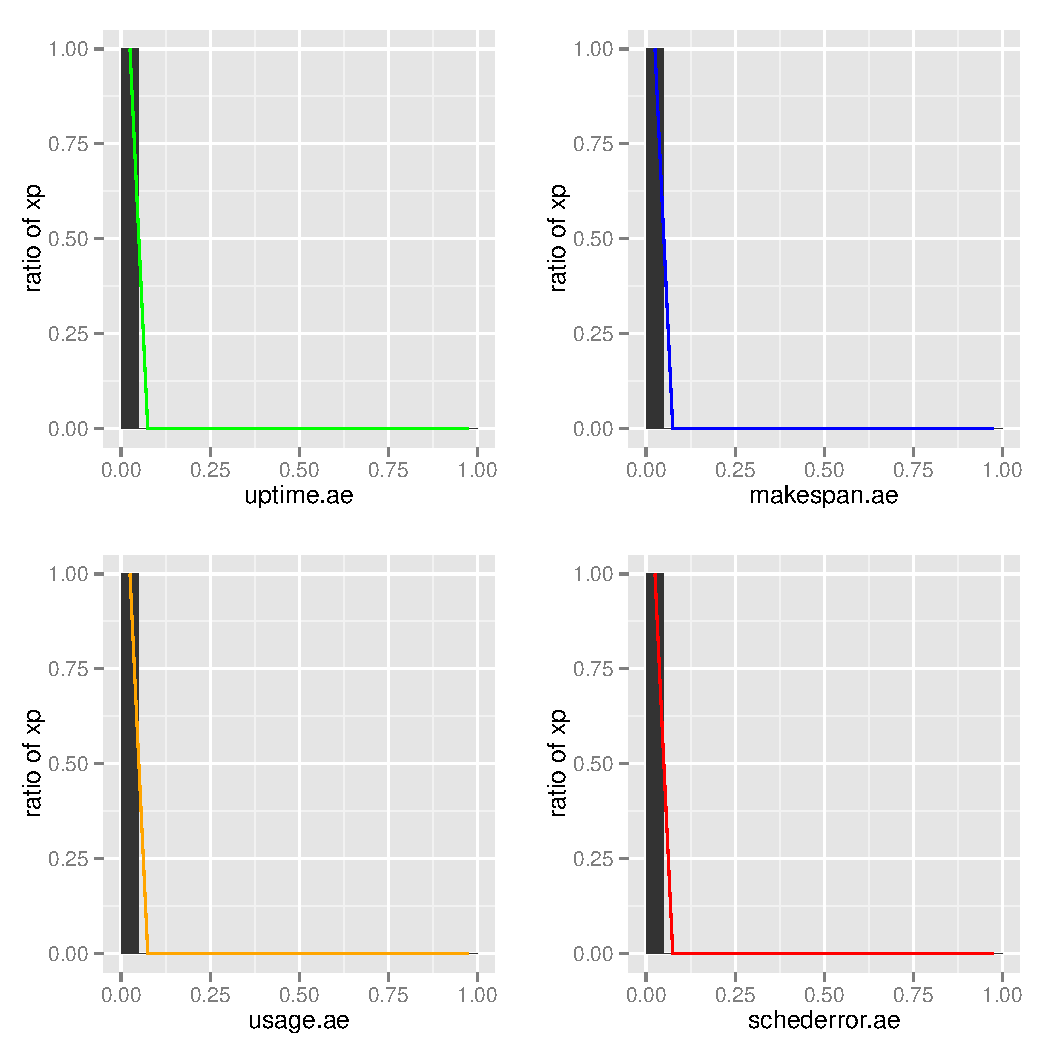
\includegraphics[width=\textwidth]{sim_best-openstack-icps-omssa-noschederror-4metrics.pdf}

  \input{\vrpath sim_best-openstack-icps-omssa-noschederror-4metrics-mmmm.latex}
      
  \input{\vrpath sim_best-openstack-icps-omssa-noschederror-4metrics-mmmm-cmp.latex}

\caption{Frequencies and statistics about absolute error of best simulations for openstack-icps / 
ommssa, without scheduling error cases (91 xps)}
\end{figure}       

      Filtering the xps showing clocks-related issues (16 xps), the results are perfect:
      all metrics present a mean ae of at most $0.001$.
      
      %Worst-case: v3.standard.hrt.asap.regular.openstack-icps.2
      The less accurate simulation shows a makespan absolute error of $0.010$. 
      Actually, the makespan of the simulation is $94s$, whereas it is $95s$ in reality.
      This small difference is due to one lag between two consecutive tasks 
      in the middle of the simulation. Such lags are not injected in our simulations.
      
      This shows that, providing that one can inject the right information, 
      the only limitation of our simulator are micro clock-related hazards.
      
      
 \item openstack-icps / montage (36 xps): 
 
      \input{\vrpath sim_best-openstack-icps-montage-4metrics-mmmm.latex}

      \input{\vrpath sim_best-openstack-icps-montage-4metrics-mmmm-cmp.latex}

      With a work-flow, scheduling errors are more numerous 
      (ae mean of $0.24$ for a max of $0.79$), leading to less accurate assessments
      of uptime, makespan and usage (mean ae of $0.01$, $0.05$, and $0.01$), that
      is ten times more than with a BoT.
      
      First, montage has much more tasks (from 43 to 1672) than omssa (from 33 to 223).
      Consequently, queues are much longer, which increases the clock-related issues.
      
      Second, BoT scheduling are actually made offline (i.e. scheduling decisions are taken
      before any actual execution), while WF scheduling implies decisions during 
      the execution, every time dependencies are satisfied. 
      Those decisions rely on the system state (predicted end date of nodes for 
      instance). Consequently, divergences between simulation and reality have
      more important impacts with WF than with BoTs.
      
      %Worst case: v3.standard.3x3.afap.regular.openstack-icps.1 
      %first proverror: 2mass_pleiades_2x2_gather
      %Log of schlouder shows that all solutions are elligible, 
      %but it shouldn't be this one (which is in the middle of the queue)... Mystery!
      
      For instance, the worst case shows a very large amount of scheduling errors 
      (0.954). A close examination of this case shown that the simulation behave
      as expected : After the first dependencies were satisfied,
      three newly ready tasks $t1$, $t2$, and $t3$ were scheduled on the node $n$.
      However in reality, scheduling takes time. During this time, the last task
      scheduled to node $n$ was completed between the scheduling of $t2$ and $t3$, 
      but before $t1$ were actually submitted to $n$. This lead to mistakingly 
      set the state of node $n$ to idle, impacting the scheduling decision of $t3$.
      
      Those kind of complex and unforeseeable events are actually frequent 
      when confronted to reality. However, they are utterly difficult to detect
      (1672 jobs were scheduled for the presented case).
      Comparing real execution with simulation allow the detection of such case, 
      without having to look at each scheduling decision.
      
      the last task assigned to node $n$ was 
      completed during the scheduling of the tasks which dependencies were satisfied 
      first. But those tasks were intended to 
      This completion lead 
      Schlouder to mistake the state of the 
      
      
 
 \item bonfire / omssa (75 xp): 
 
      \input{\vrpath sim_best-bonfire-omssa-4metrics-mmmm.latex}
      
      \input{\vrpath sim_best-bonfire-omssa-4metrics-mmmm-cmp.latex}
      
      On a public shared heterogeneous cloud, scheduling errors are more numerous 
      (AR mean of $0.03$ for a max of $0.86$), leading to less accurate assessments
      of uptime, makespan and usage (mean AR of $0.005$, $0.045$, and $0.053$).

      More interesting, usage are never perfectly assessed: 
      16\% of xp show less than $0.05$ of AR, 
      while 86\% show an AR between $0.05$ and $0.10$
      
      This show the impacts of public heterogeneous platforms on simulation
      accuracy: 
      It is not possible to precisely simulate the vm-to-pm scheduling algorithm of 
      public cloud, as they are generally not public, and their decisions impacts 
      performances, as one can not predict the power of the VM one get.
 
 \item bonfire / montage (56 xp): 
 
      \input{\vrpath sim_best-bonfire-montage-4metrics-mmmm.latex}
      
      \input{\vrpath sim_best-bonfire-omssa-4metrics-mmmm-cmp.latex}
 
      On a public shared heterogeneous cloud, scheduling errors are even more numerous 
      (AR mean of $0.48$ for a max of $0.96$), leading to less accurate assessments
      of uptime, makespan and usage (mean AR of $0.10$, $0.115$, and $0.48$).
      
      This is simply explained by the cumulation of inaccuracies from 
      both platform and applications. 
\end{itemize}



\subsection{Boottime impacts}

Assessing the impact of efficient boottimes simulation.

Same simulations, without injecting the boottimes observations. 
Thus, boottimes are only predictions, based on linear regressions of previously
observed boottimes.

\begin{figure}
  \centering
  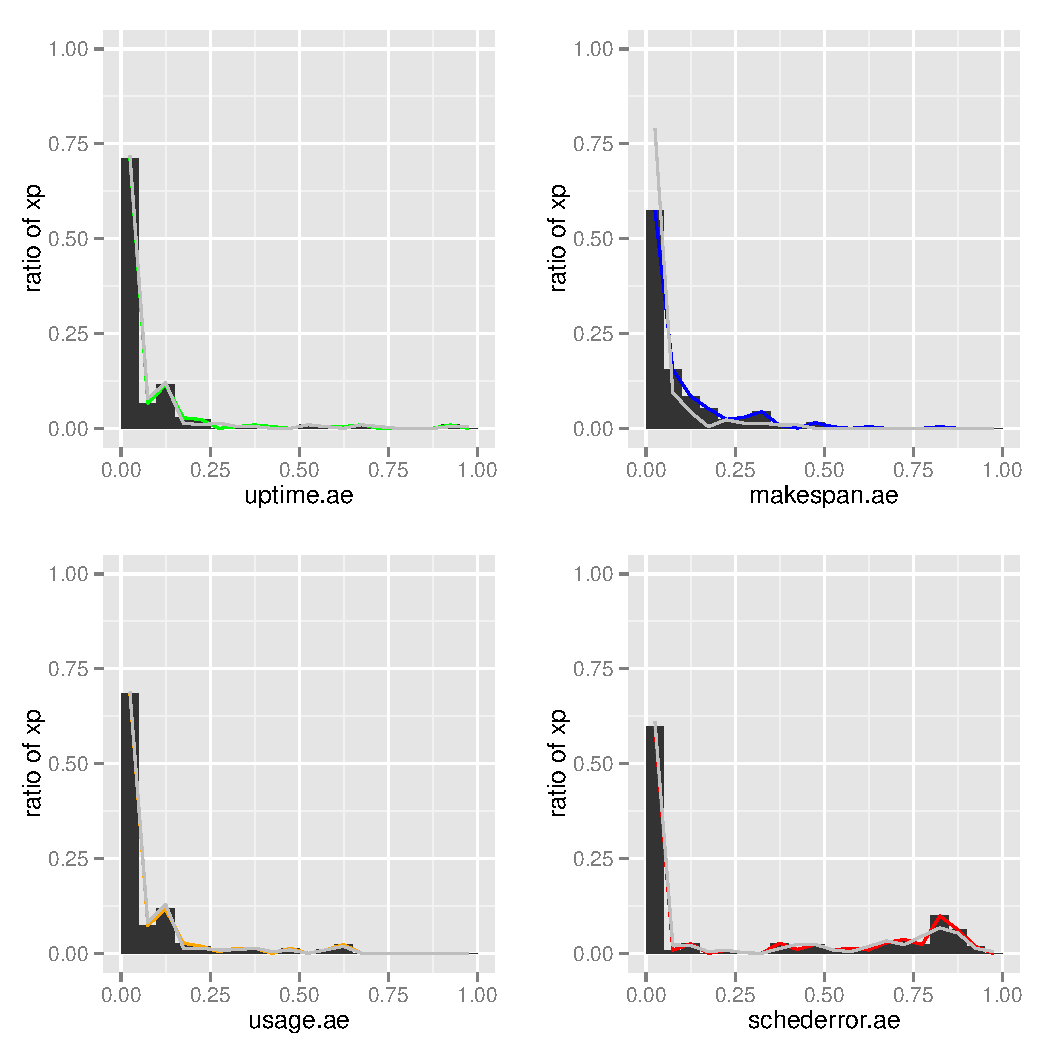
\includegraphics[width=\textwidth]{sim_no-boottimes-4metrics-cmp.pdf}

  \input{\vrpath sim_no-boottimes-4metrics-mmmm.latex}

  \input{\vrpath sim_no-boottimes-4metrics-mmmm-cmp.latex}

  \input{\vrpath sim_no-boottimes-4metrics-mmmm-twobytwo.latex}

  \caption{Frequencies, statistics, and comparison with best of simulations with no real boot times 
  injection}

\end{figure} 

%worst case: v3.standard.2x2.asap.regular.fr-inria.2 
The worst case show a makespan ae of $0.816$ (3141s instead of 17076s). 
This is due to boottimes on BonFire that were completely of charts: 
5 boots were normal (ranging from 232s to 311s), 
the 17 others ranged from 3281s to 11084s.
Whereas BonFire were intended to deliver 22 simultaneous VMs, only 5 were available
at the time of the experiment. Instead of refusing the following 17 VMs, the
provisioning system of BonFire put them in pending state, waiting for the delivered
ones to stop. The VMs being provisioned for one hour, following the 5 normal boots, 
5 boots took approximatively 1 hour, then 5 other boots took 2 hours,
and 5 another more took 3 hours. Finally, 2 boots took 1 hour after the last 
dependencies were satsified.

This illustrates that defective clouds can not be efficiently simulated without 
proper information capture. However, once captured, this kind of defection is
perfectly simulated by SchIaaS. Consequently, it can be used to assess behavior 
and robustness of solutions facing these defections.

%Best case: v3.standard.3x3.afap.regular.de-hlrs.2
Some case are surprisingly improved without the real boot times injection:
For instance, one xp shows a real makespan of 25788s, for 35106s with boot times
injection and 24266s without. 




\subsubsection{No-threads}

Injection of: real boot times and some times due to Schlouder internal threads, 
such as lapses after a node become ready and the start of the first job.

Assess the impact of efficient internal threads simulation

\begin{figure}
  \centering
  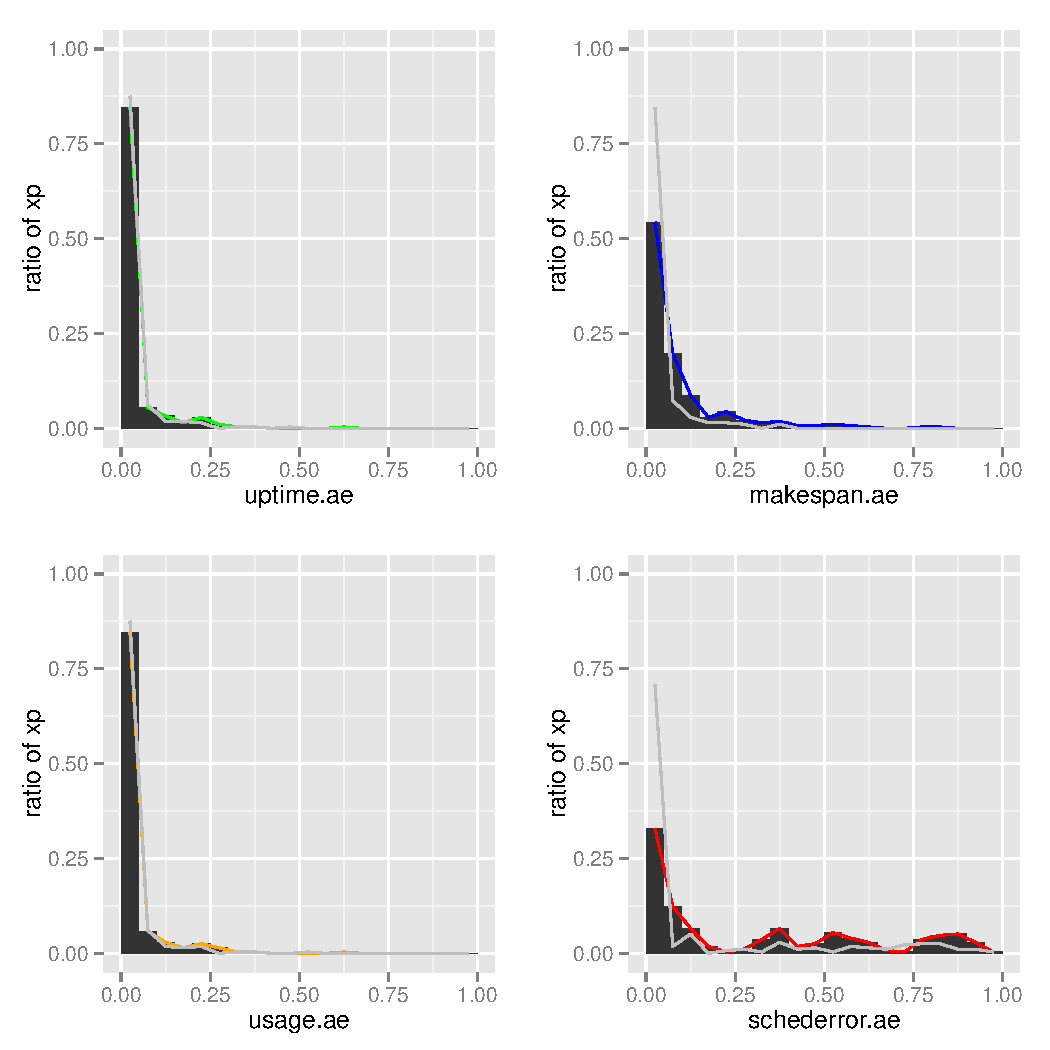
\includegraphics[width=\textwidth]{sim_no-threads-4metrics-cmp.pdf}
  
  \input{\vrpath sim_no-threads-4metrics-mmmm.latex}

  \input{\vrpath sim_no-threads-4metrics-mmmm-cmp.latex}

  \input{\vrpath sim_no-threads-4metrics-mmmm-twobytwo.latex}
    
  \caption{Frequencies, statistics, and comparison with best of simulations with no real thread times
  injection}
\end{figure} 



\subsubsection{Communications}

Injection of: real boot times, some times due to Schlouder internal threads, 
such as lapses after a node become ready and the start of the first job, 
and, real runtimes and real data size for jobs input and output communications.

Assess the impact of efficient communications 

\begin{figure}
  \centering
  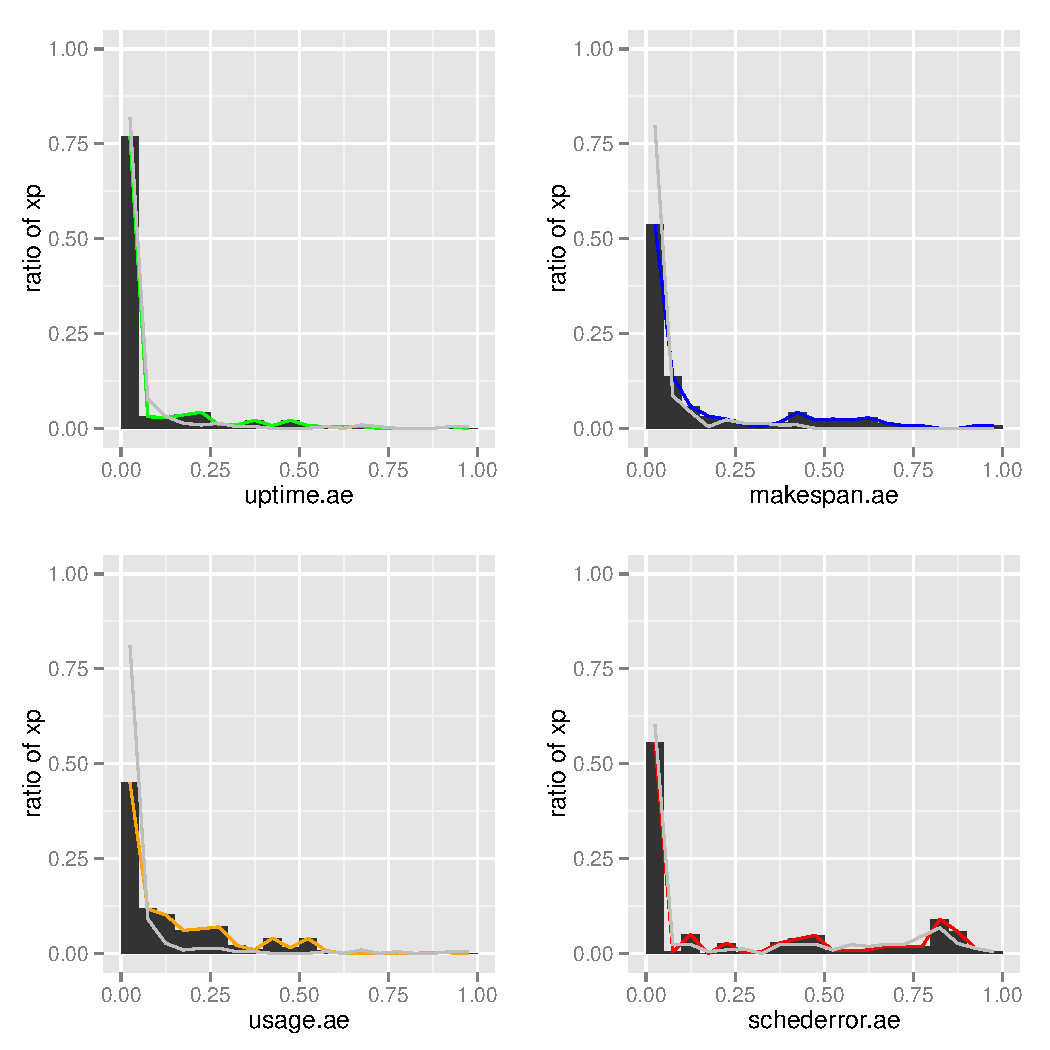
\includegraphics[width=\textwidth]{sim_communications-4metrics-cmp.pdf}
  
  \input{\vrpath sim_communications-4metrics-mmmm.latex}

  \input{\vrpath sim_communications-4metrics-mmmm-cmp.latex}

  \input{\vrpath sim_communications-4metrics-mmmm-twobytwo.latex}

  \caption{Frequencies, statistics, and comparison with best of simulations with simulation of communications}
\end{figure} 

\begin{figure}
  \centering
  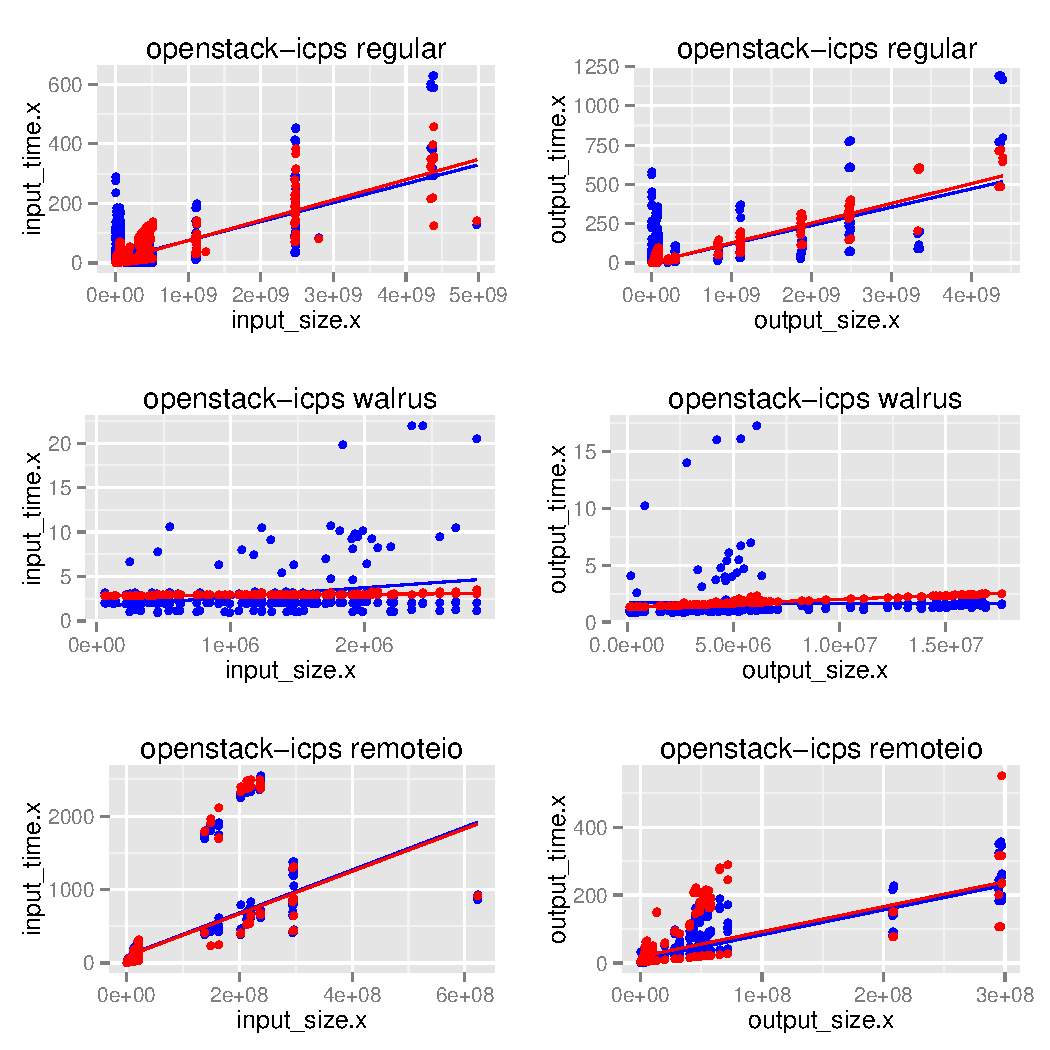
\includegraphics[width=\textwidth]{communications-openstack-icps.pdf}
  
  \caption{Linear regressions of communication times vs. data size, 
    according to platform, storage, and communication direction on openstack-icps}
\end{figure} 


\begin{figure}
  \centering
  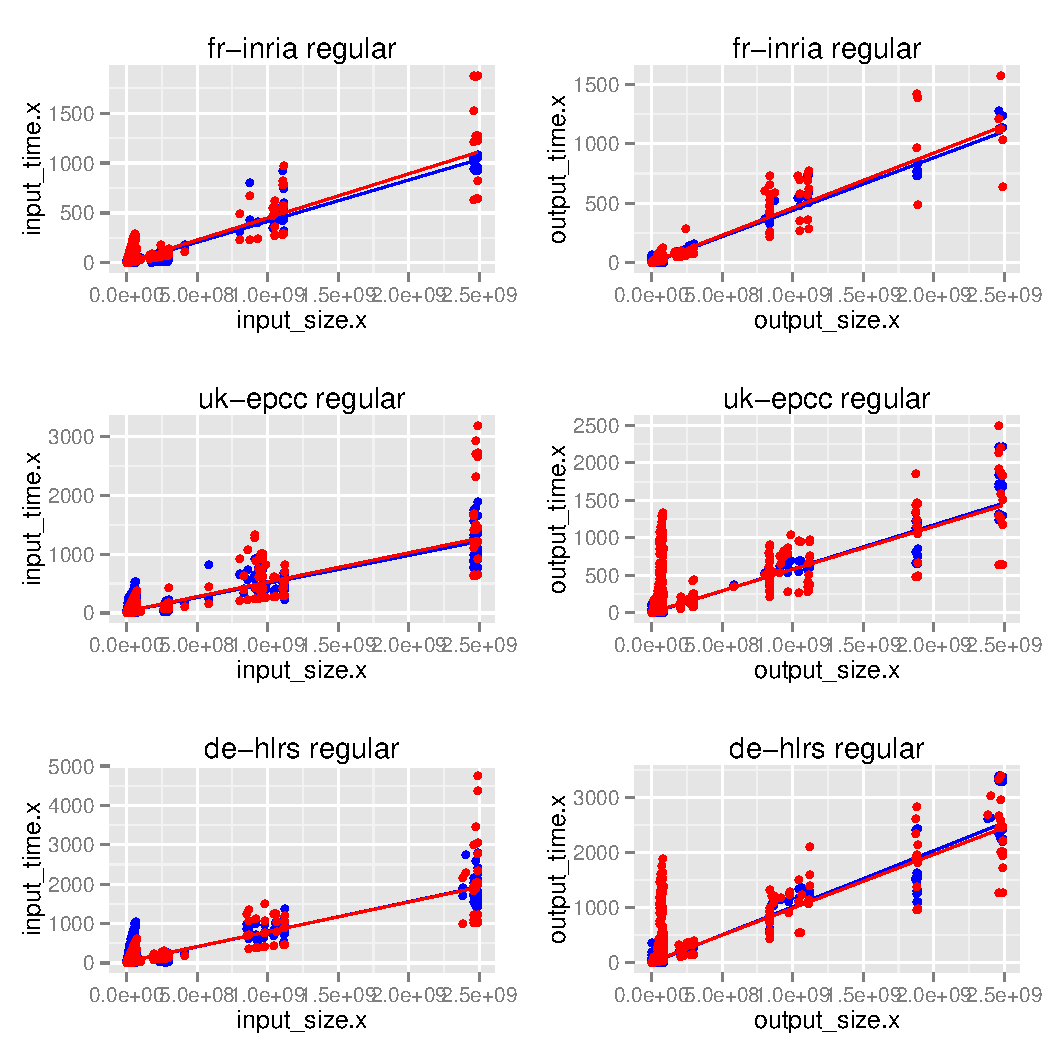
\includegraphics[width=\textwidth]{communications-bonfire.pdf}
  
  \caption{Linear regressions of communication times vs. data size, 
    according to platform, storage, and communication direction on BonFire}
\end{figure} 


\subsubsection{Prediction}

Injection of nothing from the real xp, except the xp description as submitted 
to schlouder.

Assess the efficiency of using a simulator as a predictor of a cloud.

\begin{figure}
  \centering
  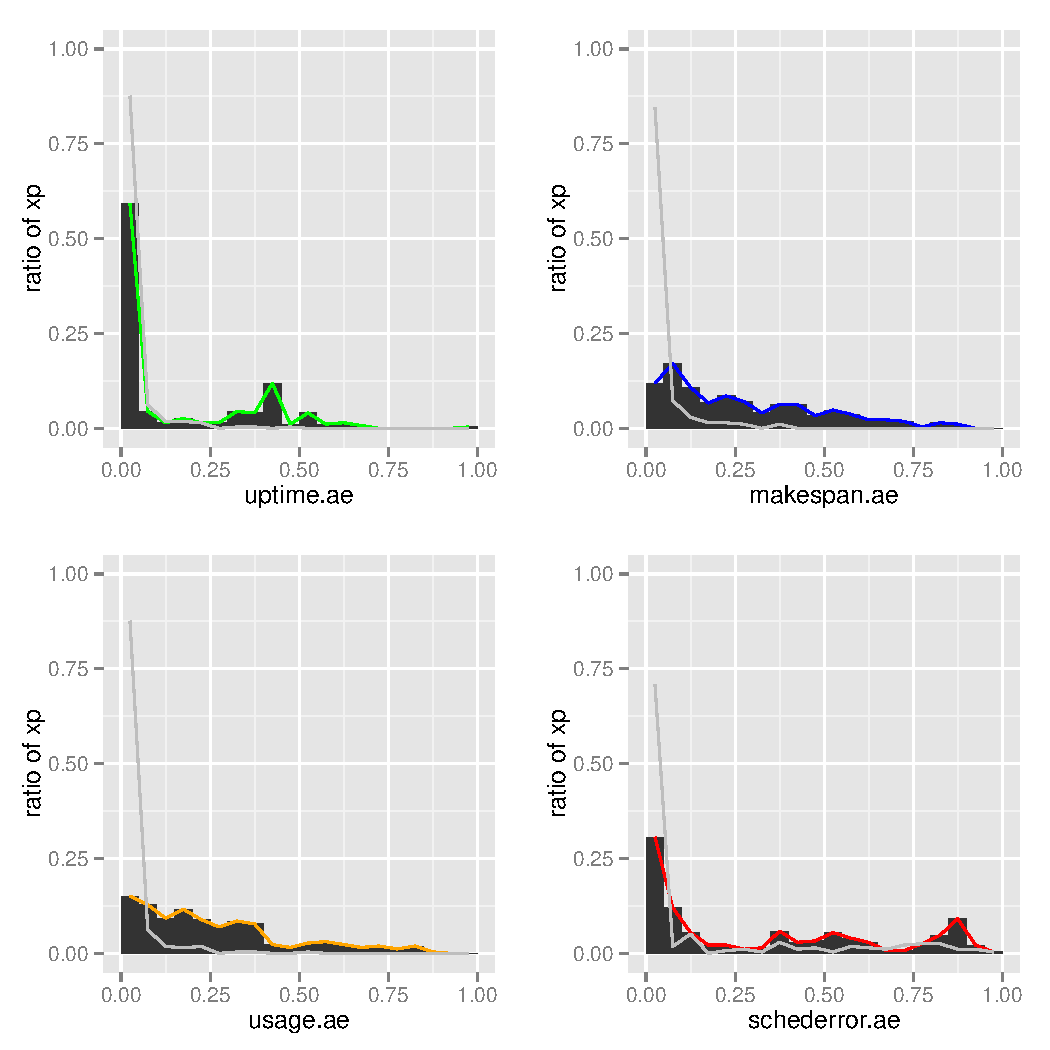
\includegraphics[width=\textwidth]{sim_predictions-4metrics-cmp.pdf}
  
  \input{\vrpath sim_predictions-4metrics-mmmm.latex}

  \input{\vrpath sim_predictions-4metrics-mmmm-cmp.latex}

  \input{\vrpath sim_communications-4metrics-mmmm-twobytwo.latex}

  
  \caption{Frequencies, statistics, and comparison with best of simulations with no injection}
\end{figure} 

\section{Open-science}

\begin{verbatim}
git clone https://git.unistra.fr/gossa/schlouder-traces.git
git clone https://scm.gforge.inria.fr/anonscm/git/schiaas/schiaas.git 
cd schiaas
cmake .
make
cd lab
./lap.py -p2 setup/simschlouder/validation.cfg
cd setup/simschlouder/validation-results
ls
\end{verbatim}



\bibliographystyle{plain}
\bibliography{biblio}

\end{document}


